\chapter{Introducción}
\label{chapter:introduccion}

%%% SECTION
\section{Título}

Análisis predictivo del comportamiento de los clientes en sus interacciones con la empresa.
 
 
%%% SECTION
\section{Palabras clave}

\begin{itemize}
    \item Predictive analytics  
    \item User interactions 
    \item Customer experience 
\end{itemize}

%%% SECTION
\section{Resumen de la propuesta}

Los clientes interactúan con las empresas a través de diversas formas de comunicación (teléfono, web, aplicaciones móviles, redes sociales, e-mails...). La finalidad de estas comunicaciones puede ser por distintos motivos, como por ejemplo: 

\begin{itemize}
  \item Obtener información de productos y precios.
  \item Consultar la facturación.
  \item Hacer reclamaciones por cualquier problema con su servicio.
  \item Contratar nuevos productos o servicios.
  \item Modificar cualquier condición de los contratos existentes.
  \item Dar de baja el propio contrato.
\end{itemize}

Las empresas suelen disponer de un sistema CRM en donde se gestionan las interacciones con los clientes, tanto los propios como los potenciales. 

Una funcionalidad importante de estos sistemas, es que permiten recopilar información de los distintos canales. 

En el caso de las grandes empresas que cuentan con millones de clientes el procesamiento de todos estos datos puede ser muy complejo y lento, pero existen tecnologías de procesado masivo como la computación paralela que permiten reducir el tiempo considerablemente. 

Todo este historial de interacciones con los usuarios puede ser analizado posteriormente para comprender sus preferencias y necesidades, de modo que las empresas pueden mejorar las relaciones comerciales con sus clientes y por lo tanto ofrecer una mejor experiencia del cliente. 

Así pues, se puede hacer uso de algoritmos de Inteligencia Artificial y \textit{``Machine Learning"} para influir en la toma de decisiones de la empresa. Por ejemplo, este análisis predictivo puede provocar un aumento de las ventas cruzadas y de la retención de clientes. Además, todas estas mejoras podrían repercutir en la reducción de los costes operativos derivados del impacto de las llamadas telefónicas al centro de llamadas. 


%%% SECTION
\section{Justificación}

Existen diversos canales para la comunicación entre las empresas y sus clientes, como pueden ser el teléfono, la web, las aplicaciones móviles, las redes sociales o los correos electrónicos. Aunque todos estos canales no ofrecen las mismas funcionalidades, muchas tareas se pueden realizar desde varios canales.

En la actualidad muchas empresas están enfocando sus esfuerzos a usar cada vez más la estrategia de contenidos ``omnichannel", que pretende mejorar la experiencia de usuario. El objetivo de esta estrategia es orquestar los múltiples canales de comunicación para que se integren y cooperen entre ellos.

Todos estos servicios suponen un coste para la empresa, pero es la plataforma telefónica la que más gastos implica. Esto parece lógico, pues con unos cuantos servidores web puedes atender a múltiples peticiones a la vez, mientras que una persona puede atender una única llamada de los clientes a la vez.

Así pues, podemos suponer que un mayor uso de las plataformas digitales implicará una reducción en las llamadas y por lo tanto estaremos reduciendo costes. Es por esto que se quiere realizar un análisis en el que se pueda estudiar la relación entre el uso de la web y las aplicaciones móviles con las llamadas telefónicas.

Sin embargo, este mayor uso de las plataformas digitales aumentará significativamente la cantidad de información que es almacenada por las interacciones de los clientes. Estos volúmenes de datos suponen un problema frecuente, pues hacen casi inviable el uso de bases de datos tradicionales para extraer información. Por suerte en la actualidad existen tecnologías denominadas \textit{``Big Data"}, que son capaces de procesar masivamente datos gracias a la computación paralela.

Para comprender el comportamiento de los usuarios cuando interactúan con las plataformas digitales, tales como la web de clientes o las aplicaciones móviles, ya existen herramientas muy potentes que proporcionan todo tipo de analíticas de uso, pero por desgracia estas herramientas no son capaces incorporar la información que se puede obtener de las llamadas telefónicas.

Por este motivo, el disponer distintas fuentes de datos implicará la necesidad de tener un proceso de ETL con el cual conseguiremos integrar todos estos datos en un mismo repositorio, de forma que los datos posteriormente puedan ser analizados. El proceso ETL cuenta con las siguientes fases:
\begin{itemize}
  \item Extracción: Extraer datos de múltiples fuentes como ERP, CRM, ficheros con formatos varios (xls, csv, xml).
  \item Transformación: Transformar estos datos en la estructura que hayamos definido en nuestro repositorio destino. El paso de transformación, incluye acciones de validación sobre reglas de negocio, validaciones técnicas (duplicados, integridad, nulos, ...), normalización y homogeneización de códigos, cambios de formato, así como costosos procesos de ordenación, filtrados, cruces y agregados.
  \item Carga: Carga de datos en las estructuras de almacenamiento final. Este paso puede ser realizado en procesos por lotes y pueden ser de diferentes tipos: por lotes, registro a registro, cargas totales, cargas incrementales, etc...
\end{itemize}

Es por todo esto que, ante la carencia de funcionalidad de las herramientas de analítica web y los problemas que acarrea trabajar con volúmenes de datos, se pretende realizar un estudio de analítica predictiva, en la que gracias a los sistemas de \textit{``Big Data"} y al uso de modelos predictivos, podamos extraer conocimiento de toda esta información y que pueda ser de ayuda en las futuras tomas de decisiones.

%%% SECTION
\section{Motivación}

Este proyecto considero que es apropiado para tratarlo como mi TFM ya que abarca varias áreas de conocimiento estudiadas a lo largo del Máster de Ciencia de Datos. Por ejemplo, está directamente relacionado con las asignaturas “Análisis de datos en entornos Big Data” y “Arquitectura de bases de datos no tradicionales”. 

Además, la temática de este TFM me parece muy adecuada, ya que está ligada a mi actual puesto de trabajo y se tratará de resolver una problemática real de la empresa.  

Por otra parte, la realización de este proyecto me permitirá adquirir nuevas habilidades profesionales, pues aprenderé a trabajar en entornos \textit{``Cloud"}, mejoraré mis conocimientos de Python, seré capaz de segmentar de forma eficiente los clientes de la empresa... Todo esto poniendo en práctica la metodología \textit{``Agile"}, que hasta el momento no había tenido ocasión de usar. 

En cuanto lo personal, estudiar y aprender cosas nuevas siempre me ha ilusionado porque me permite crecer y superarme día a día. Puedo decir que para mí es como una afición, es por esto que decidí estudiar el Máster de Ciencia de Datos en la UOC. También puedo decir que cursar el resto de asignaturas ha significado cumplir un reto para mí, porque no es fácil compaginar los estudios con la vida profesional y personal. Aunque sé que realizar el TFM va a requerir muchas horas de trabajo, considero que trabajar en una materia que te apasiona lo hace mucho más sencillo. En definitiva, espero afrontar el TFM con la misma con la ilusión que he tenido durante el resto del máster.

%%% SECTION
\section{Hipótesis}

La inclusión o mejora del acceso de ciertas solicitudes comunes en los canales digitales permitirá reducir el número de llamadas recibidas en el centro de llamadas.


%%% SECTION
\section{Objetivos}

El objetivo principal será determinar qué funcionalidades en las plataformas digitales permiten la reducción de llamadas telefónicas recibidas.

En cuanto a los objetivos parciales que se pretenden conseguir son los siguientes: 
\begin{itemize}
    \item Entender la información resultante de la navegación de las plataformas digitales y relacionarla con los datos de la plataforma telefónica.
    \item Ser capaces de predecir el canal por el que se ha realizado una reclamación.
    \item Ser capaces de predecir qué clientes tienen activada la facturación electrónica.
    \item Visualización de resultados.
\end{itemize}


%%% SECTION
\section{Metodología}
En este apartado vamos a describir la estrategia de investigación y la metodología de trabajo que se va a seguir durante el desarrollo del TFM.

\subsection{Estrategia de investigación}

La estrategia que se empleará a lo largo del desarrollo de este proyecto será \textit{''Action research”}\cite{oates}. Este es un proceso cíclico iterativo compuesto de las siguientes fases:
\begin{itemize}
    \item Diagnóstico: Identificar la naturaleza de la situación del problema, incluyendo todos los factores interrelacionados, y desarrollar una teoría de trabajo sobre la situación y como puede ser cambiada. 
    \item Planificación: Especificar acciones que puedan aliviar la situación 
    \item Intervención: Tomar las acciones en las áreas de aplicación acordadas.
    \item Evaluación: Establecer si los efectos teóricos de la acción fueron realizados, y si estos realmente mitigaron el problema. 
    \item Reflexión: Decidir lo que se ha logrado tanto en términos de resultados prácticos como de nuevos conocimientos, y si se requiere un nuevo ciclo de investigación-acción.
\end{itemize}

\subsection{Metodología de trabajo}

La metodología de trabajo que se empleará en este proyecto será Scrum\cite{sutherland}, una de las metodologías ágiles más usadas en la actualidad\cite{ellis}. 

Scrum es un proceso de gestión de proyectos. Se utiliza más a menudo en conjunto con el desarrollo de nuevos programas informáticos. El proceso de Scrum implica el uso de equipos autodirigidos que eligen una tarea de una lista de scrum predeterminada y trabajan en esa tarea hasta que se completa. El proceso permite que los proyectos complejos se dividan en secciones manejables y se trabaje en ellos de manera eficiente y oportuna. Cuando el proceso de Scrum se sigue completamente, la productividad se incrementa hasta en un 400 por ciento. Sin embargo, la implementación de sólo algunos aspectos del proceso generalmente resulta en fracaso. Algunas industrias fuera del desarrollo de software también han comenzado a implementar variaciones de scrum. 
Las características básicas de esta metodología son las siguientes: 
\begin{itemize}
    \item Se trabaja en iteraciones de 1 a 4 semanas, donde se debe acabar con un producto entregable. En nuestro caso será de 2 semanas. 
    \item El equipo es auto organizado, los coordinadores y clientes deben trabajar en todo momento con el equipo de desarrollo, facilitando las tareas y resolviendo dudas. Gracias al uso de videoconferencias y correo electrónico se conseguirá tener una comunicación fluida con el tutor. 
    \item Se deben tener unos requisitos perfectamente priorizados reflejando el valor del negocio. 
    \item Se debe mantener un ritmo de trabajo constante, permite que no haya descuidos y retrasos en el sprint. 
\end{itemize}

Los roles implicados son los siguientes: 
\begin{itemize}
    \item Product owner: Se corresponde con el dueño del producto. 
    \item Scrum master: Es el coordinador del equipo, controla al equipo para la consecución de los objetivos.  
    \item Team: Desarrolladores del producto. 
\end{itemize}

En nuestro caso, intentaremos aproximarnos lo máximo posible a esta metodología, aunque tendremos que hacer alguna excepción ya que el equipo será únicamente de dos personas, tomando el tutor la figura de \textit{``Product owner"} y el estudiante los perfiles de equipo y \textit{``Scrum master"} simultáneamente. 

Cabe destacar que este proyecto va a ser realizado íntegramente en un solo entorno, por lo que no se van a realizar despliegues en producción. En consecuencia, no será necesario seguir ninguna metodología de puesta en producción, tal y como pueda ser el sistema de entrega continua DevOps\cite{walls}.


%%% SECTION
\section{Planificación del proyecto}

La planificación del proyecto está supeditada a los plazos de entrega fijados para las diferentes prácticas de evaluación continua. Dentro de cada práctica se han detectado una serie de tareas cuyos plazos se muestran en el siguiente diagrama. 

\subsection{Diagrama de Gantt}
\begin{figure}[H]
\centerline{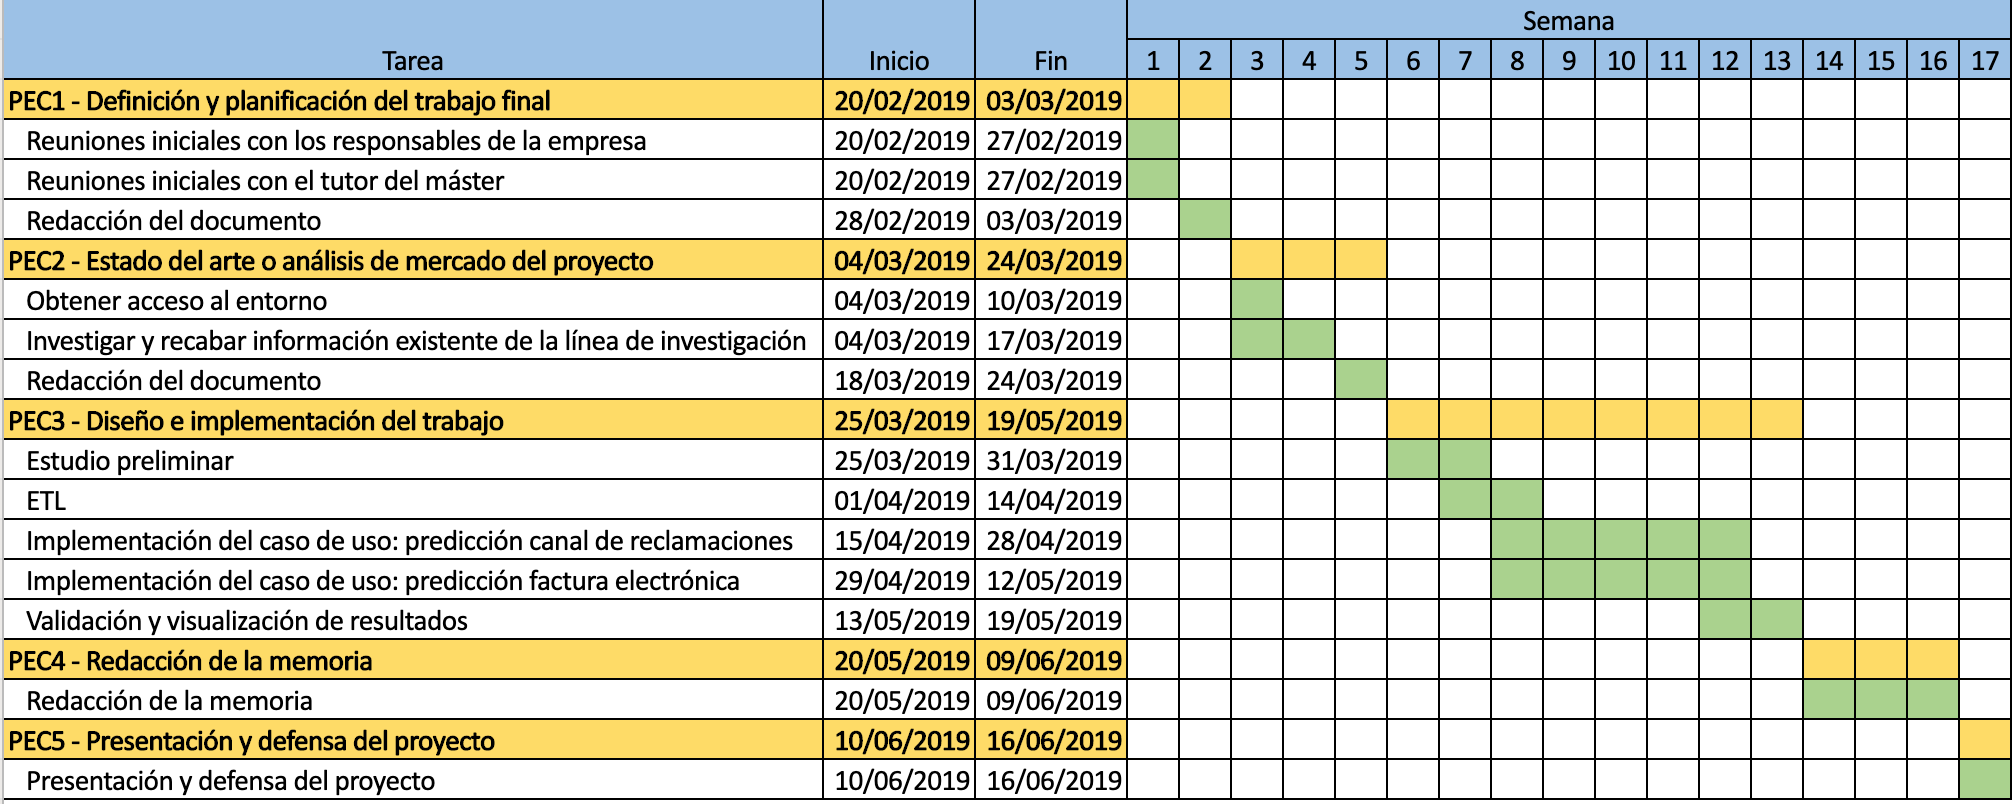
\includegraphics[width=1.0\textwidth]{TFM/figs/planificacion.png}}
\caption{Diagrama de Gantt que muestra la planificación del TFM}
\label{fig:planificacion}
\end{figure}

\subsection{Control de riesgos} 

Se han identificado dos riesgos potenciales que, por factores internos o externos, pueden alterar el curso de la planificación realizada para este TFM.  

Estos son los siguientes: 
\begin{itemize}
    \item Retraso en la obtención de accesos a la plataforma de \textit{``Big Data"}:
    
En el caso que no se disponga de la plataforma para la fase de “Diseño e implementación del trabajo”, se tomará la medida que eliminará tarea de implantación del caso de uso “Modelos de segmentación”. 
    \item Imposibilidad de poder aprovisionar información de clientes por motivos de GDPR:

Dado este caso, se tratará de hacer la segmentación de los clientes únicamente a partir de sus datos geopolíticos y de sus consumos.
\end{itemize}
